\documentclass{scrartcl}
\usepackage[utf8]{inputenc}

\title{University of North Carolina at Charlotte}
\subtitle{Introduction to Robotics: Lab 2}
\author{Alex Boyd and Edgar Joya}
\date{June 2014}

\usepackage{natbib}
\usepackage{graphicx}
\usepackage{mathtools}
\usepackage{listings}
\usepackage{float}

\begin{document}

\maketitle
\tableofcontents

\addsec{Overview}
The purpose of this experiment is to familiarize the student with LabView and to introduce the robot used for the course.

LabVIEW is a programming language that uses a graphical interface to create programs. Each 
program created using LabVIEW is called a VI. A subVI is similar to a function call and is 
simply a program within another program. There are two windows the front panel and block 
diagram. The front panel displays the controls, graphs, and indicators of the program. The block 
diagram shows the mechanisms of the program such as the control structures like case 
statements, for loops, while loops, math operations, subVIs, and the wiring done for all 
components. 
The robot is already assembled and ready to be programmed. No major modifications to the 
robot, in terms of mechanical additions or to the electronic components, are necessary. Minor 
additions may need to be made in later labs. The robot consists of a single board RIO (sbRIO) 
FPGA board with pins on top in order to easily attach new sensors to the robot whenever needed. 
The chassis holds the motors of the robot and hides the multitude of wires inside. 
The sensor that is attached to the front of the robot is a type of sensor called an ultrasonic sensor. 
The name of this sensor is the Parallax PING ultrasonic range sensor. This sensor, shown below 
in Figure 1, sends out an ultrasonic pulse. The distance is measured by the sensor by measuring 
the time for the echo to return. The Parallax PING ultrasonic range sensor incorporates an 
activity status LED and has one I/O pin. 

\addsec{Objectives}
\begin{itemize}
\item To write a program which sets up the Parallax PING ultrasonic sensor.

\item To write a program which allows remote control of the direction of the Parallax PING ultrasonic sensor on a  rotational axis. 

\item To write a program which makes the led lights on the back of the DaNi robot blink at any rate specidied by the user.
\end{itemize}

\addsec{Program 1 - Parallax Ping Ultrasonic Sensor}
When creating the first program, the instructions were followed from the lab. Following "Creating your first VI" instructions, the application was named MyFirstApp.vi which can be found at the the public github repository by following the following command on a linux terminal if you have git installed:
\begin{lstlisting}
git clone git@github.com:eujc21/ECGR-4161.git
\end{lstlisting}
The results for this simple program is depicted by the following image:
\begin{figure}[H]
  \centering
    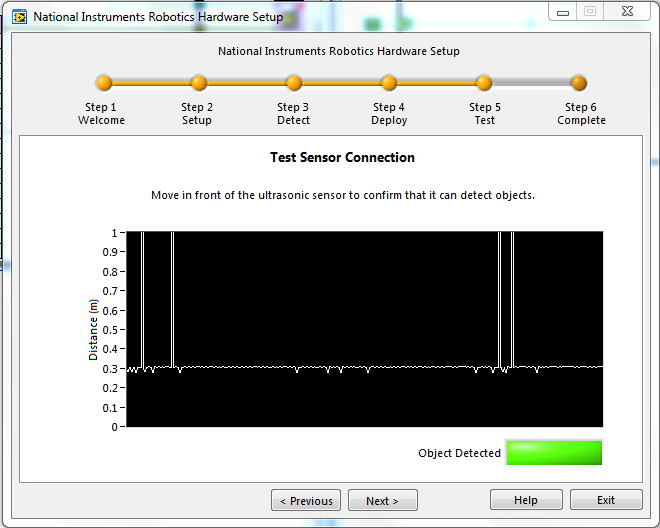
\includegraphics[width=1\textwidth]{configuration_setup.png}
    \caption{First Program Set Up.}
    \label{fig:first}
\end{figure}

Figure  ~\ref{fig:first}  shows the LabView process in which the robot is initialized and prepared for using the Ultrasonic Ping Sensor
This excercise shows how much of the process to program is now automated. The ease of user-friendly software that helps setting up a  connection to a robot. Also configuring this robot to control and read back from a a sensor. This type of instant feedback is a big help when it comes to debugging.

\addsec{Program 2 - Manipulating a Servo for direction of Ultrasonic Sensor}
The second program was created again by following the instructions in the lab manual. A couple of things had to be analyzed for this part of the lab.

The response time had to be manipulated for a faster response of the servo motor. This was easily accomplished by changing the time of the loop from $$1000ms$$ to $$100ms$$

Another manipulation for creating this program was to manipulate degrees into radians, the conversion equation for this manipulation is the following:
$$\frac{\pi}{180}\times \text{degrees}=\text{radians}$$

Figure ~\ref{fig:second} displays the block diagram, after saving and compiling this program, Figure ~\ref{fig:third}  displays the interface in which the servo is now accessible for control to move in the parameters given. The parameters that this servo is given is limited by $90^\circ$. The Waveform in Figure ~\ref{fig:third} shows the sensitivity of the Ultrasonic Ping Sensor. When the amplitude is high, it means that a surface is closer to the sensor than when the amplitude is low. This was tested by placing an object and passing it by the sensor.

\begin{figure}[H]
  \centering
    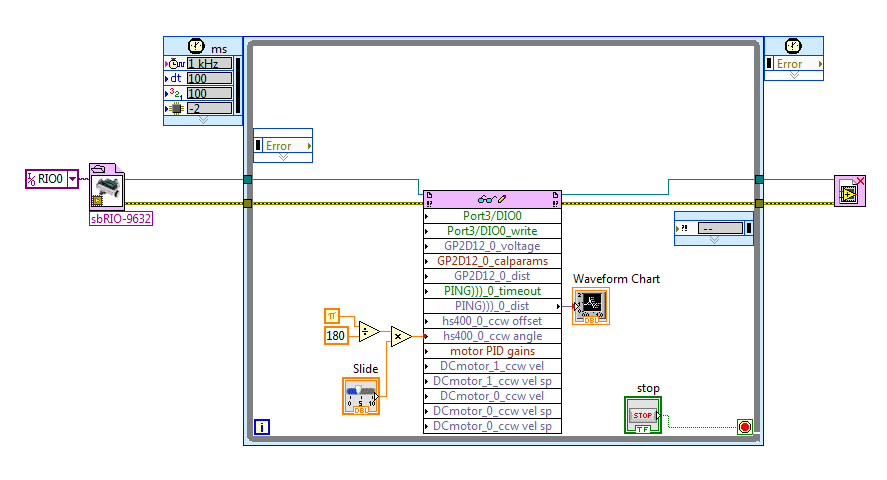
\includegraphics[width=1\textwidth]{servo_block.png}
    \caption{Ultrasonic Ping Sensor and Servo Block Diagram}
    \label{fig:second}
\end{figure}

\begin{figure}[H]
  \centering
    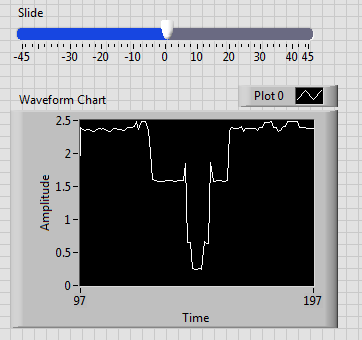
\includegraphics[width=1\textwidth]{graph2.png}
    \caption{Interface for UPSS}
    \label{fig:third}
\end{figure}

\addsec{Program 3 - First FPGA Application}
The third program was created again by following the instructions in the lab manual.This program controls the frequency of the LED display. With this program the LED display had to be changed to a lower frequency which can be seen by the naked eye. Figure ~\ref{fig:fourth} displays the block diagram for the LED logic. In this figure, the frequency is controlled by the block labeled count.


\addsec{Conclusion}
All the files can be found in the following repository. \citep{github}. 
\begin{figure}[H]
  \centering
    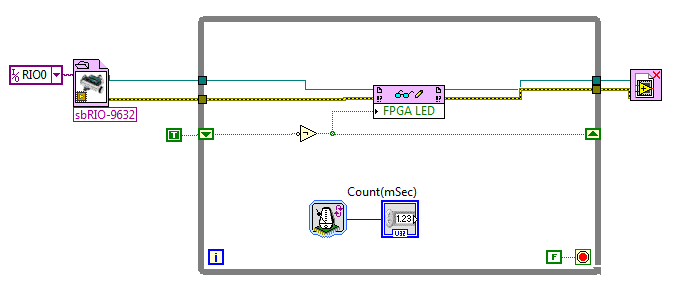
\includegraphics[width=1\textwidth]{fpga.png}
    \caption{FPGA Block Diagram}
    \label{fig:fourth}
\end{figure}

\listoffigures
\bibliographystyle{plain}
\bibliography{references}
\end{document}
